%%% Template originaly created by Karol Kozioł (mail@karol-koziol.net) and modified for ShareLaTeX use

\documentclass[a4paper,12pt]{article}

\usepackage[T1]{fontenc}
\usepackage[utf8]{inputenc}
\usepackage{graphicx}
\usepackage{xcolor}

\renewcommand\familydefault{\sfdefault}
\usepackage{tgheros}


\usepackage{url}
\usepackage{enumerate}

\usepackage{amsmath,amssymb,amsthm,textcomp}
\usepackage{enumerate}
\usepackage{multicol}
\usepackage{tikz}

\usepackage{geometry}
\geometry{left=25mm,right=25mm,%
bindingoffset=0mm, top=20mm,bottom=20mm}


\linespread{1.3}

\newcommand{\linia}{\rule{\linewidth}{0.5pt}}

% custom theorems if needed
\newtheoremstyle{mytheor}
    {1ex}{1ex}{\normalfont}{0pt}{\scshape}{.}{1ex}
    {{\thmname{#1 }}{\thmnumber{#2}}{\thmnote{ (#3)}}}

\theoremstyle{mytheor}
\newtheorem{defi}{Definition}

% my own titles
\makeatletter
\renewcommand{\maketitle}{
\begin{center}
\vspace{2ex}
{\huge \textsc{\@title}}
\vspace{1ex}
\\
\linia\\
\@author \hfill \@date
\vspace{4ex}
\end{center}
}
\makeatother
%%%

% custom footers and headers
\usepackage{fancyhdr}
\pagestyle{fancy}
\lhead{}
\chead{}
\rhead{}
\lfoot{Projectlet puzzle}
\cfoot{}
\rfoot{Page \thepage}
\renewcommand{\headrulewidth}{0pt}
\renewcommand{\footrulewidth}{0pt}
%

% code listing settings
\usepackage{listings}
\lstset{
    language=Python,
    basicstyle=\ttfamily\small,
    aboveskip={1.0\baselineskip},
    belowskip={1.0\baselineskip},
    columns=fixed,
    extendedchars=true,
    breaklines=true,
    tabsize=4,
    prebreak=\raisebox{0ex}[0ex][0ex]{\ensuremath{\hookleftarrow}},
    frame=lines,
    showtabs=false,
    showspaces=false,
    showstringspaces=false,
    keywordstyle=\color[rgb]{0.627,0.126,0.941},
    commentstyle=\color[rgb]{0.133,0.545,0.133},
    stringstyle=\color[rgb]{01,0,0},
    numbers=left,
    numberstyle=\small,
    stepnumber=1,
    numbersep=10pt,
    captionpos=t,
    escapeinside={\%*}{*)}
}

%%%----------%%%----------%%%----------%%%----------%%%

\begin{document}

\title{Puzzle}

\author{rs@toprllc.com}

\date{\today}

\maketitle

\section*{Introduction}

In this projectlet, we study the classic \textbf{Game of Fifteen} (\url{https://en.wikipedia.org/wiki/15_puzzle}). Apart from the numerous avenues for theoretical studies, this affords the practising engineer special challenges as well.

\paragraph{UI} This requires a fairly simple user interface. Implementation will only have to identify and deal with mouse clicks and very little else.

\paragraph{Abstraction} The variations of this game span different sizes of the puzzle i.e. 4x4, 5x5 and so on. Thus this is an introduction to parametrising the implementation.

\paragraph{Variation} We will introduce a variation in this projectlet namely instead of numbered tiles, a supplied image is used. Thus solution then requires the original image to be reproduced by sliding the individual tiles according to the stated rules.

\section*{Specification}

Based on the above broad ideas, the following specifications will guide the exploration.

\paragraph{Choice of faces} The number of tiles and an image file in a standard format like png or jpg are the basic parameters to an implementation. The user should be allowed to dynamically change the tile face.

\paragraph{User commands} The user shall be able to approach the puzzle in a different ways. Starting with a jumbled puzzle, the user can slide the tiles to produce the solution. Alternatively starting with a solution, the tiles can be manually jumbled to produce interesting patterns.

\paragraph{Graphic libraries} Quite a few GUI libraries are available to choose from. E.g. \url{https://www.gtk.org/} is a platform, language agnostic choice. So is \url{https://www.qt.io/} though with more licensing restrictions. There are more language specific choices as in \textbf{fyne} (\url{https://fyne.io/}) which may be very \textbf{go} specific. \textbf{Dotnet} \url{https://dotnet.microsoft.com/} rounds out this list as a whole platform including user interfaces.

\section*{Implementation}

\subsection*{Challenges}

\paragraph{Concurrency Model} The gtk library specifies that all changes to the GUI be performed from a single thread of execution. Others such as fyne do not have such an explicit specification. In this example, since every action in the puzzle is driven by the user - by mouse clicks or button presses, the design is quite simple. Except when we need to update the think time which counts up independently.

\paragraph{Image manipulation} The need to support images as tile faces exposes us to some basic image processing needs eg to crop, recombine images. More interesting however will be the investigation of the marriage between the static image representation in files (.png or .jpg) and the more dynamic GUI environment and the widget sets presented by the library.

\paragraph{Mouse Clicks}  Mouse clicks are the way the sliding tiles are identified. Each library supports a different way of identifying mouse clicks and their position. 

\paragraph{Algorithm Hiding} In order to experiment with different GUI libraries, the algorithmic aspects need to be isolated and a clean interface established.

\subsection*{Example Project}

An example project has been developed to illustrate the concepts - with the following specifications:

\paragraph{}
\fbox{%
    \parbox{6in}{%

usage: puzzle [no of segments] [imagename] [fyne|gtk]\\
       use . for segments=4 as well as etc/flower.png
     }%
}

\paragraph{}

An implementation in \textbf{go} language has been developed using fyne and gotk3 bindings to gtk \url{https://github.com/gotk3/gotk3} and is available for exploration and enhancements. 

\fbox{%
    \parbox{5in}{%
     \url{https://ToprLLC@bitbucket.org/ToprLLC/puzzle.git}
    }%
}

\subsection*{Implementation with fyne graphical library}
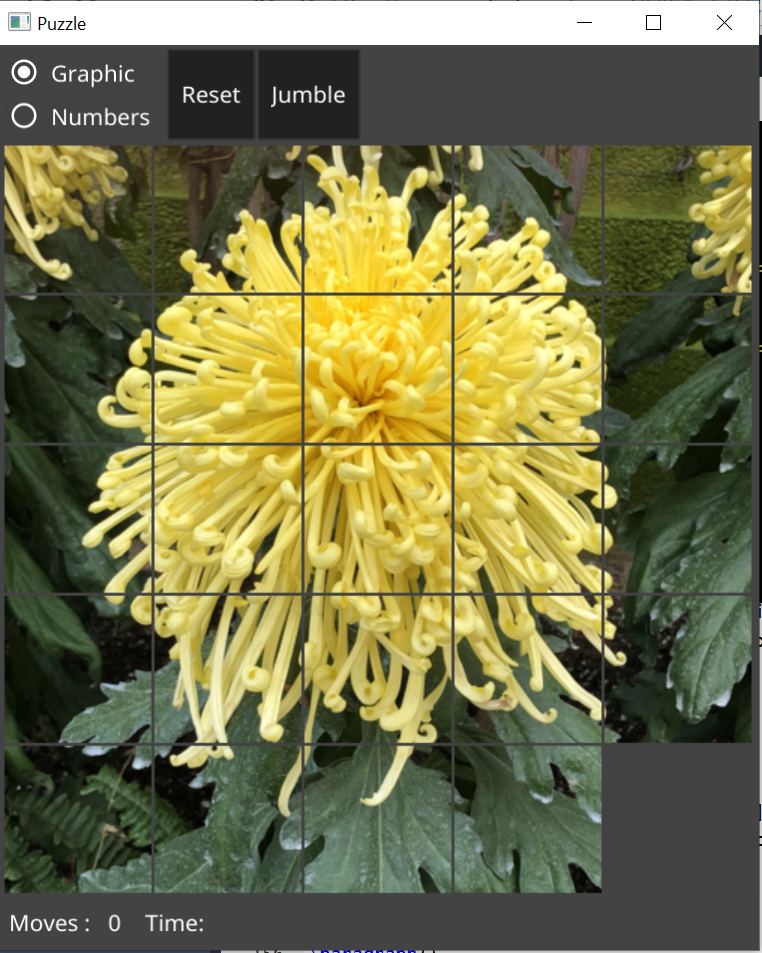
\includegraphics[width=6in]{fyne_5_begin.png}

\subsection*{Implementation with gtk - Jumbled puzzle}
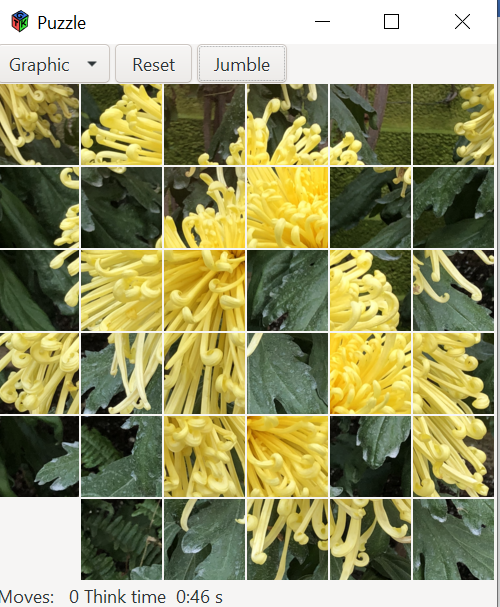
\includegraphics[width=6in]{gtk_6_jumbled.png}

\section*{Potential Improvements}

\paragraph{Undo} Keep track of each move and be able to retract.
\paragraph{Patterns} Instead of random Jumbles, arrange them in a different predictable pattern. For instance, in the equivalent numeric view, the numbers will be placed along the periphery clockwise and so on eventually with the last empty tile being close to the center.
\paragraph{Solver} Include a solver which finds the best solution from a given state presenting an animated view.
\end{document}
